\documentclass[12pt, letterpaper, titlepage]{article}

\usepackage{amsmath}
\usepackage{booktabs}
\usepackage{amsthm}
\usepackage{graphicx}
\usepackage[margin=1in]{geometry}
\usepackage{hyperref}
\hypersetup{colorlinks = true, linkcolor = blue, citecolor=blue, urlcolor = blue}
\usepackage{natbib}
\usepackage{enumitem}
\usepackage{setspace}

\usepackage[pagewise]{lineno}
\linenumbers*[1]
% %% patches to make lineno work better with amsmath
\newcommand*\patchAmsMathEnvironmentForLineno[1]{%
 \expandafter\let\csname old#1\expandafter\endcsname\csname #1\endcsname
 \expandafter\let\csname oldend#1\expandafter\endcsname\csname end#1\endcsname
 \renewenvironment{#1}%
 {\linenomath\csname old#1\endcsname}%
 {\csname oldend#1\endcsname\endlinenomath}}%
\newcommand*\patchBothAmsMathEnvironmentsForLineno[1]{%
 \patchAmsMathEnvironmentForLineno{#1}%
 \patchAmsMathEnvironmentForLineno{#1*}}%

\AtBeginDocument{%
 \patchBothAmsMathEnvironmentsForLineno{equation}%
 \patchBothAmsMathEnvironmentsForLineno{align}%
 \patchBothAmsMathEnvironmentsForLineno{flalign}%
 \patchBothAmsMathEnvironmentsForLineno{alignat}%
 \patchBothAmsMathEnvironmentsForLineno{gather}%
 \patchBothAmsMathEnvironmentsForLineno{multline}%
}

\makeatletter
\newcommand*{\Xbar}{}%
\DeclareRobustCommand*{\Xbar}{%
  \mathpalette\@Xbar{}%
}
\newcommand*{\@Xbar}[2]{%
  % #1: math style
  % #2: unused (empty)
  \sbox0{$#1\mathrm{X}\m@th$}%
  \sbox2{$#1X\m@th$}%
  \rlap{%
    \hbox to\wd2{%
      \hfill
      $\overline{%
        \vrule width 0pt height\ht0 %
        \kern\wd0 %
      }$%
    }%
  }%
  \copy2 %
}
\makeatother


\newcommand{\jy}[1]{\textcolor{blue}{JY: #1}}

\title{On Misuses of the Kolmogorov–Smirnov-Test}

\author{Anthony Zeimbekakis and Jun Yan\\
\href{mailto:anthony.zeimbekakis@uconn.edu}{\nolinkurl{anthony.zeimbekakis@uconn.edu}}\\
Department of Statistics, University of Connecticut}
\date{April 21, 2022}

\begin{document}
\maketitle

\doublespace

\begin{abstract}
The Kolmogorov-Smirnov (K-S) test is one the most popular goodness-of-fit tests for 
comparing a sample with a hypothesized parametric distribution. Nevertheless, it has 
often been misused. The standard one-sample KS test applies to independent, continuous 
data with a hypothesized distribution that is completely specified. It is not uncommon, 
however, to see in the literature that it was applied to dependent, discrete, or 
rounded data, with hypothesized distributions containing estimated parameters. 
For example, it has been “discovered” multiple times that the test is too conservative 
when the parameters are estimated \citep[e.g.,][]{Steinskog}. This paper aims to survey 
the misuses of the KS test, demonstrate their consequences through simulation, and 
provide remedies as needed.
\end{abstract}


\hypertarget{sec:intro}{%
\section{Introduction}\label{sec:intro}}

The Kolmogorov-Smirnov (K-S) statistic is one of the most popular goodness-of-fit 
tests for comparing a sample with a hypothesized parametric distribution. The test is 
performed as follows. Let $X_1, ..., X_n$ be i.i.d. random variables from $F_{n}(x)$,
the empirical cumulative distribution.
Let $F(x)$ be the population cumulative distribution. The K-S 
statistic is 
\[
  d = \max{\lvert F_{n}(x) - F(x) \rvert}.
\].
The null hypothesis is that the observations $X_1, ..., X_n$ are from the specified distribution $F(x)$, and the 
alternate hypothesis is that the data is not from $F(x)$. The table of critical 
values for $d$ are given by \citet{Massey} for various sample sizes $n$ and significance 
levels $a$. If the value of $d$ exceeds the test's corresponding critical value, 
the null hypothesis is rejected.

However, the test is often misused. The standard one-sample K-S test applies to 
independent, continuous data with a hypothesized distribution that is completely specified. 
Often in literature, it has been "discovered" that the test loses its power when 
applied to dependent or discrete data with hypothesized distributions containing 
estimated parameters. In the case of estimated parameters, \citet{Steinskog} 
demonstrates the change in power when using estimated parameters and stress caution in 
using the K-S test in such ways. \citet{Lilliefors} shows 
that using the standard table when values of the mean and standard deviation are 
estimated obtains extremely conservative results. This is supported by \citet{Capasso}, which 
concludes that failing to re-estimate the parameters may lead to wrong, overly-conservative 
approximations to the distributions of goodness-of-fit test statistics based on the empirical 
distribution function. \citet{Capasso} also notes that the impact of this possible mistake 
may turn out to be dramatic and does not vanish as the sample size increases. Remedies are provided 
by \citet{Genest} and \citet{Babu} in the form of bootstrap. \citet{Genest} provides validity 
for using parametric bootstrap with various goodness-of-fit tests. \citet{Babu} details 
the bootstrap procedure for goodness-of-fit tests and notes that both parametric and 
non-parametric procedures lead to correct asymptotic levels, however there is a correction 
required for the non-parametric case. In the case of dependent data, \citet{Durilleul} demonstrates
that the K-S statistic is too liberal for medium-to-high positive autocorrelation values. 
\citet{Durilleul} also shows that for negative autocorrelation values, the behavior is 
asymmettrical with respect to positive values. For remedies, \citet{Weiss} provides a 
procedure that is applicable specifically for data modeled by the second-order auto-regressive (AR) 
process where the parameters are known. \citet{Lanzante} tests various strategies for dealing with 
temporal dependenceand concludes that a test based on Monte-Carlo simulations performed the best.
We propose a bootstrap procedure involving copulas to account for dependence.

The purpose of this paper is to expand on the misuses of the K-S test and propose 
solutions in the case that the K-S test would still like to be used. In order to set 
up the demonstrations, simulated data is used throughout. Unless otherwise specified, 
the random data is generated from a standard normal distribution with sample size $n = 100$. 
Therefore the cumulative distribution $F(x)$ of the K-S test for much of this paper is standard normal.

\hypertarget{sec:fitted}{%
\section{Fitted Parameters}\label{sec:fitted}}

The K-S test shows significant issues in the case of fitted parameters. One assumption 
of the K-S test is that the hypothesized distribution is completely specified. 
However, the procedure is sometimes performed where the population cumulative 
distribution $F(x)$ has parameters $\mu=\Xbar$, the sample mean, and $\sigma^2=s^2$, 
the sample variance \citep{Lilliefors}. This case is demonstrated in Figure~\ref{fig:hist_fitted} 
under the Naive plot. The naive K-S test was performed by estimating the parameters 
of $F(x)$ using the fitted distribution of the sample data. Since the data is generated 
from a standard normal distribution with seemingly all assumptions met, a uniform 
distribution of $U(0,1)$ is expected for the p-values. However this is under the 
assumption that the K-S test holds its power, which it no longer does due to using 
fitted parameters. Therefore, there is notable deviation from the uniform distribution. 

To resolve this problem, both parametric and non-parametric bootstrap can be performed. 
The bootstrap procedure is as follows. 

\begin{itemize}
  \item 
    Let $X_1^*,...,X_n^*$ be i.i.d random variables from $\hat{F}_n$, an estimator 
    of the distribution function $F_n$ based on the sample $X_1,...,X_n$
  \item 
    Let $\hat{\theta}_n^* = \theta_n(X_1^*,...,X_n^*)$, where $\theta$ is the 
    parameter vector and $\hat{\theta}_n$ represents the sample mean and variance 
    of the sample $X_1,...,X_n$
  \item 
    $\hat{\theta}_n^*$ represents the sample mean and variance of the bootstrap 
    sample $X_1^*,...,X_n^*$
  \item Thus, the K-S statistic for each bootstrap case is $\max(\lvert F(x)-F^*_n(x) \rvert)$
\end{itemize}

In parametric bootstrap, the resampling is done where $\hat{F}_n = F(.;\hat{\theta}_n)$. 
Bootstrap samples are drawn from ${F}(.,\hat{\theta}_n)$ where the assumed distribution 
$F$ is normal and $\hat{\theta}_n = (\Xbar, s)$, the sample mean and sample standard 
deviation. For each bootstrap sample, a K-S test statistic is found using those 
fitted parameters.

In non-parametric bootstrap, the resampling is done where $\hat{F}_n = F_n$. The non-parametric
case requires a correction for bias detailed by \citet{Babu}. There is a known bias
term $B_{n}(x) = \sqrt{n}(F_{n}(x) - F(x;\hat{\theta}_n)$. Including this term in the
calculation of the K-S statistic corrects the bias \citet{Babu}:
$d = \max\lvert F_{n}(x) - F(x) - B_{n}(x) \rvert$.

Figure~\ref{fig:hist_fitted} displays the results of from our simulations. The procedure 
is replicated $1000$ times using the standard normal distribution with sample size $n=100$. 
In each replicate test, $1000$ bootstrap samples are obtained. The p-value can be calculated
by counting the number of bootstrap K-S statistics greater than or equal to the observed K-S statistic, 
and then dividing by the number of bootstrap samples. It is clear from the figure that both
bootstrap processes correct for the problem of fitted parameters. The plots appear to be
$U(0,1)$, which is expected of a full power test.

\begin{figure}[tbp]
  \centering
  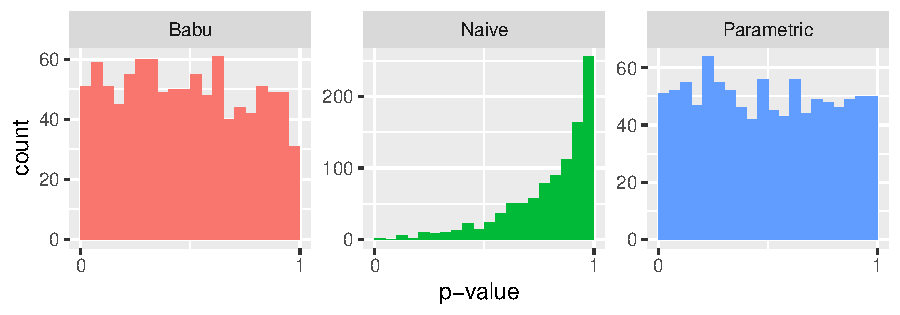
\includegraphics{hist_fitted}
  \caption{Histograms demonstrating fitted parameters.}
  \label{fig:hist_fitted}
\end{figure}

\hypertarget{sec:dependence}{%
\section{Problem under Serial Dependence}\label{sec:dependence}}

The K-S test also displays issues in the case of dependence. As mentioned, an assumption of the 
test is that the data is independent. Unfortunately, real data is often temporally
or spatially dependent and the results of a goodness-of-fit test would be valuable. 
When the K-S test is performed on dependent data it performs poorly. This is demonstrated
with a simulation in Figure~\ref{fig:hist_correlation}. Data is generated from a
first-order autoregressive model (AR(1)) with a standard normal distribution. The simulation
is done with the levels of $\psi$ varying from $(-3,3)$. The results support \citet{Durilleul}'s 
assertion that the K-S statistic is too liberal for positive autocorrelation values, and 
that the behavior is asymmettrical for negative values.

\begin{figure}[tbp]
  \centering
  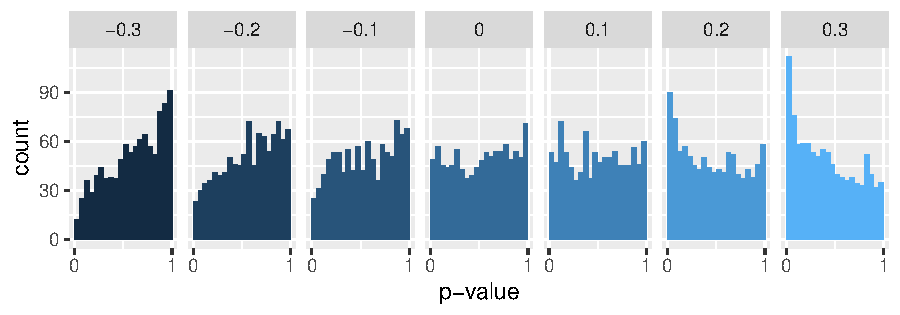
\includegraphics{hist_correlation}
  \caption{Histograms of P-values with correlated data.}
  \label{fig:hist_correlation}
\end{figure}

In order to correct this, we can employ copulas. A copula is a mechanism to form 
joined distributions. It allows us to incorporate temporal dependence while ensuring that our
marginal distribution is the same as the fitted distribution. The procedure is as follows:

\begin{enumerate}
  \item Calculate the observed K-S statistic
  \item Get the lag-1 sample auto-spearman rho
  \item Perform parametric bootstrap to get an empirical distribution of the K-S statistic
\end{enumerate}

\begin{figure}[tbp]
  \centering
  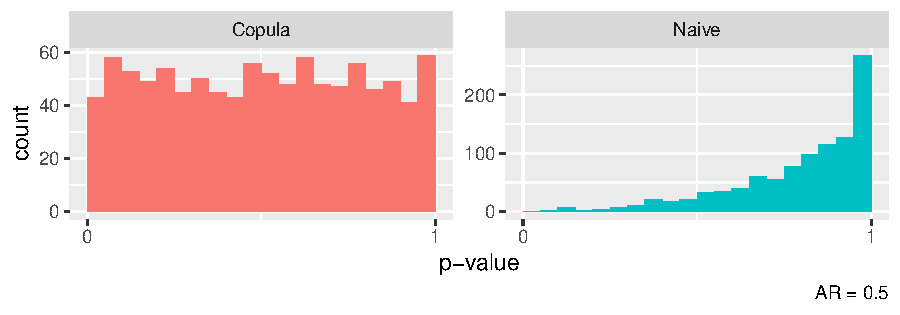
\includegraphics{hist_copula_only}
  \caption{Histograms demonstrating copula use to correct dependence.}
  \label{fig:hist_copula_only}
\end{figure}

Figure~\ref{fig:hist_copula_only} displays the results of the copula remedy for dependent data.
The data is generated from an AR(1) model with $\psi = .5$. The copula used is to model
dependence is the normal copula. $1000$ replicate tests were performed with $1000$ bootstrap samples per test.
The naive test is performed by simply using the K-S test without correcting for any 
potential dependence.

\hypertarget{sec:fittedwithdependence}{%
\section{Fitted with Dependence}\label{sec:fittedwithdependence}}

The remedy using copulas is effective in the case where both assumptions are violated.
This is shown in Figure~\ref{fig:hist_copula}. The "super naive" plot is the resulting 
p-values when you naively use fitted parameters while ignoring dependence in the data.
The "naive parametric" plot is the result of applying parametric bootstrap to correct
for fitted parameters, as done in section \ref{fitted}. Of course, the "copula" plot 
applies the fix for both assumptions.

\begin{figure}[tbp]
  \centering
  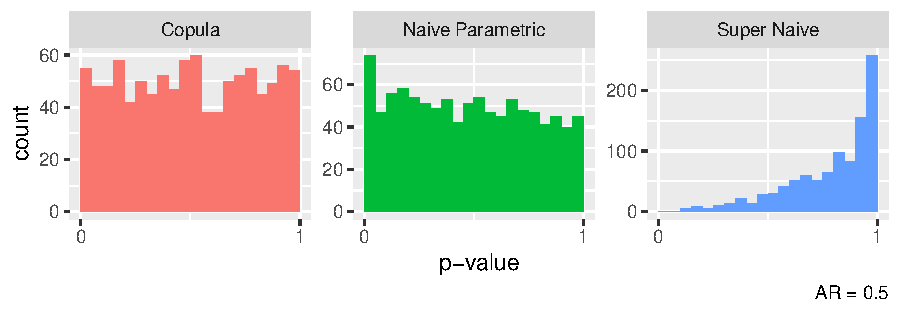
\includegraphics{hist_copula}
  \caption{Histograms demonstrating copula use to correct fitted parameters and dependence.}
  \label{fig:hist_copula}
\end{figure}

We would also like to show that copulas work for more than a simple AR(1) model. 
Figure~\ref{fig:hist_copula_ma1} is the procedure performed on data generated from 
an MA(1) model with $\theta = 0.5$. Figure~\ref{fig:hist_copula_arma} is the procedure 
performed on data generated from an ARMA(1,1) model with $\psi = 0.5$ and $\theta = 0.3$. 
It is also possible to apply our procedure to other distributions. The data in Figure~\ref{fig:hist_copula_gamma} is generated from $Gamma ~ (3,1)$ with $\rho = 0.5$.

\begin{figure}[tbp]
  \centering
  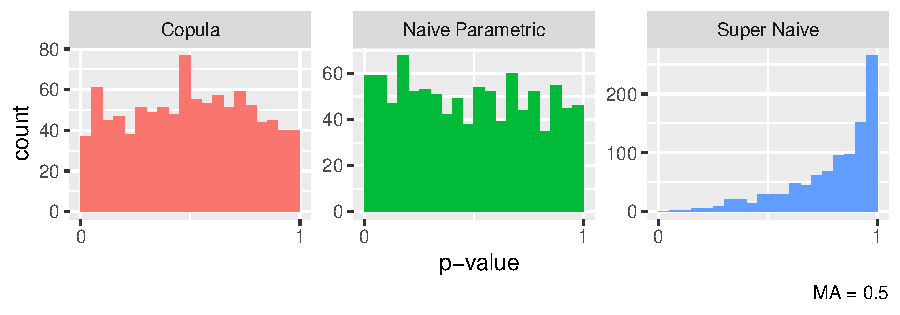
\includegraphics{hist_copula_ma1}
  \caption{Histograms demonstrating remedy use with MA(1) model.}
  \label{fig:hist_copula_ma1}
\end{figure}

\begin{figure}[tbp]
  \centering
  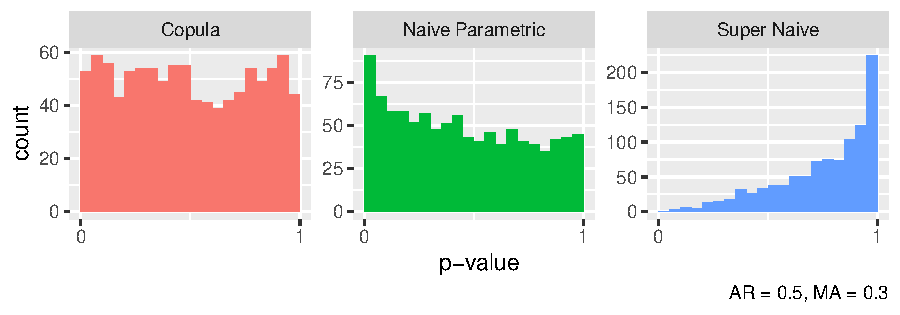
\includegraphics{hist_copula_arma}
  \caption{Histograms demonstrating remedy use with ARMA(1,1) model.}
  \label{fig:hist_copula_arma}
\end{figure}

\begin{figure}[tbp]
  \centering
  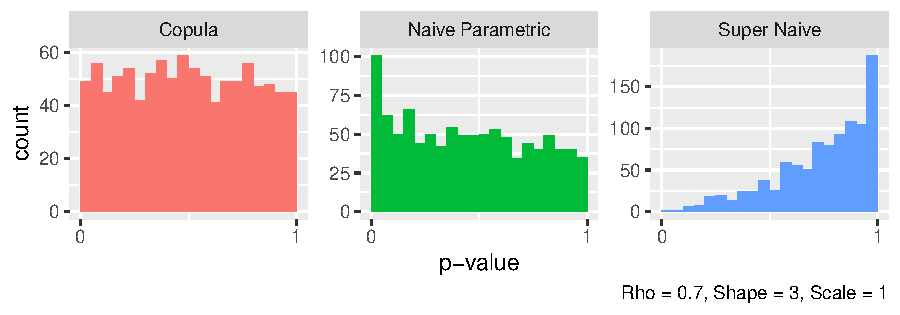
\includegraphics{hist_copula_gamma}
  \caption{Histograms demonstrating remedy with Gamma(3,1).}
  \label{fig:hist_copula_gamma}
\end{figure}

\begin{figure}[tbp]
  \centering
  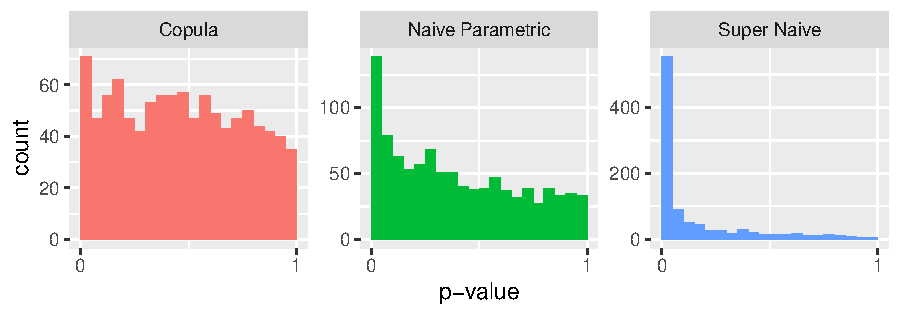
\includegraphics{hist_copula_ar2}
  \caption{Histograms demonstrating copula use to correct dependence.}
  \label{fig:hist_copula_ar2}
\end{figure}

\begin{figure}[tbp]
  \centering
  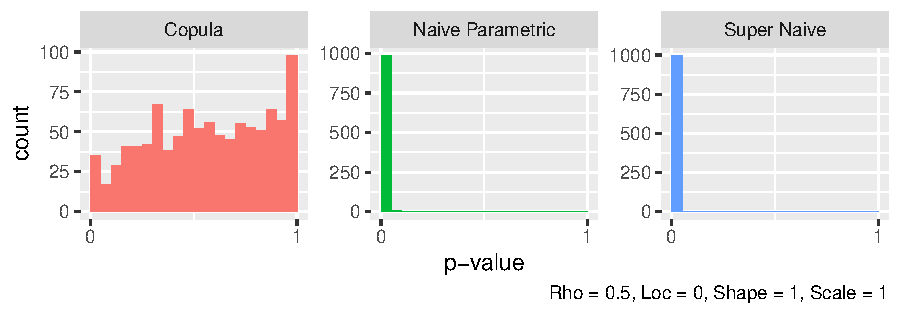
\includegraphics{hist_copula_gev}
  \caption{Histograms demonstrating copula use to correct dependence.}
  \label{fig:hist_copula_gev}
\end{figure}

\hypertarget{sec:conclusion}{%
\section{Conclusion}\label{sec:conclusion}}

The K-S test has base assumptions that the hypothesized distribution is completely specified
and the data is independent. When these assumptions are violated, the test is no
longer accurate and remedies must be performed. In the case of fitted parameters, 
parametric and non-parametric bootstrap can restore the power of the test. A bias 
correction is required if the non-parametric form is used \citep{Babu}. In the case of dependent
data, a procedure using bootstrap with copulas to model dependency shows positive results.
When both assumptions are violated, that is the case where the data has dependence and 
parameters must be fitted, the copula remedy also shows positive results. The tests were 
performed on simulated data from a standard normal distribution, though also appear effective
against other distributions such as gamma and gev. The copula remedy
is not a complete solution. Regardless of the true depedence, we use an AR(1) model.
Therefore, if the AR(1) model is a close approximation of the truth, the fix can work.
However, in cases such as AR(2), the approximation is incorrect and the fix does not 
completely restore power.


\bibliographystyle{chicago}
\bibliography{citations.bib}


\end{document}
